
\lecture{Introduction to Hypothesis Testing}{intro-to-hypothesis-testing}
\section{Introduction to Hypothesis Testing}

\title{Introduction to Hypothesis Testing}
\subtitle{Is there a difference? (yes/no)}

%\author{Kelly Black}
%\institute{Clarkson University}
\date{3 November 2014}

\begin{frame}
  \titlepage
\end{frame}

\begin{frame}
  \frametitle{Outline}
  \tableofcontents[hideothersubsections,sectionstyle=show/hide]
\end{frame}


\subsection{Clicker Quiz}


\iftoggle{clicker}{%
  \begin{frame}
    \frametitle{Clicker Quiz}

    A random variable has a mean of 3.7 and a standard deviation of
    1.2. What is the probability that a sample mean using six samples is
    more than 4.1?

    \vfill

    \begin{tabular}{l@{\hspace{3em}}l@{\hspace{3em}}l@{\hspace{3em}}l}
      A: 0.2061  & B: 0.7939  & C: 0.8165
    \end{tabular}

    \vfill
    \vfill
    \vfill


  \end{frame}
}




\subsection{Introduction To Hypothesis Testing}

\begin{frame}{The Idea}

  \vfill

  I want to take some action. I think it will be ``better.'' Is it? 

  \vfill

  This is a yes or no question!

  \vfill
  
\end{frame}

\begin{frame}
  \frametitle{Introduction To Hypothesis Testing}

  A randomly chosen can of oil should have a mean viscosity of 1.80
  centi-Stokes. I put in an additive and take fifteen random
  samples. The sample mean of the viscosities is 1.87 centi-Stokes
  with a \redText{sample} standard deviation of 0.15
  centi-Stokes. \blueText{Did it make a difference?}

  \vfill

  \only<2->%
  {
    
    \centerline{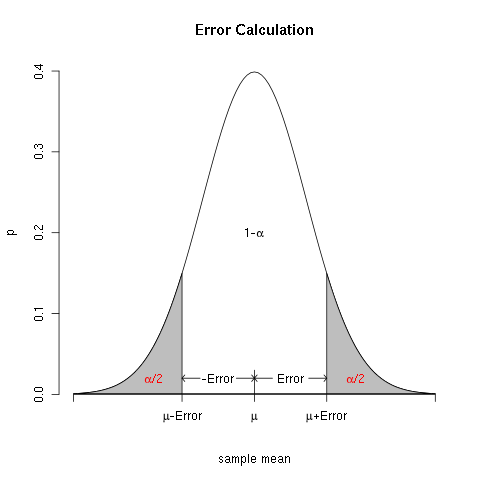
\includegraphics[width=4cm]{img/confidenceInterval}}

    \iftoggle{clicker}{%
      Clicker Quiz: \\
      \begin{tabular}{l@{\hspace{3em}}l@{\hspace{3em}}l@{\hspace{3em}}l}
        A: Yes  & B: No  & C: Maybe?
      \end{tabular}

    }

  }

  \vfill

\end{frame}


\begin{frame}
  \frametitle{The Problem}

  Situation: We think that the mean of $X$ is $\mu$ (some number).


  \begin{tabular}{ll}
    Problem: & $\bar{x}$ is a random variable. \\
    Problem: & $\bar{x}$ is our {\color{red}only way} of estimating $\mu$!
  \end{tabular}

\end{frame}

\begin{frame}{What do we do?}

  \begin{enumerate}
  \item<1-> We have some {\color{red}idea/belief} of what to expect.
  \item<2-> This is our {\color{red}hypothesis} of what we \textit{think} is happening.
  \item<3-> We want to {\color{red}make a case} for some change in how we interpret the
    situation.
  \item<4-> {\color{red}Assume} that the \textit{status quo} is good or better. (Call this the
    \textit{Null Hypothesis}, $H_0$.)
  \item<5-> {\color{red}Construct a hypothesis} about what we \textbf{think}
    is happening. (Call this the \textit{alternate hypothesis}, $H_a$.)
  \item<6-> Collect \textit{evidence} {\color{red}assuming $H_0$ is true}. 
  \item<7-> If the \textit{evidence} is {\color{red}\textit{``highly
        unlikely''} under the assumed conditions} then reject the null
    hypothesis, otherwise we cannot reject the null hypothesis.
  \end{enumerate}
  
\end{frame}

\subsection{Examples}

\begin{frame}{Hypothesis Testing}

  \begin{columns}
    \column{.5\textwidth}
    $H_0$ is the null hypothesis.
    \vfill
    \textit{This is what we think is unlikely.}
    \column{.5\textwidth}
    $H_a$ is the alternate hypothesis.
    \vfill
    \textit{This is what we think is likely.}
  \end{columns}
\end{frame}

\begin{frame}
  \frametitle{Left Sided Test of the Mean}

  \begin{columns}
    \column{0.45\textwidth}
    \textit{You think that the mean is lower.}

    Notation:
    \begin{eqnarray*}
      \begin{array}{lrcl}
        H_0: & \mu & = & \# \\
        H_a: & \mu & < & \#
      \end{array}
    \end{eqnarray*}

    \column{0.55\textwidth}

    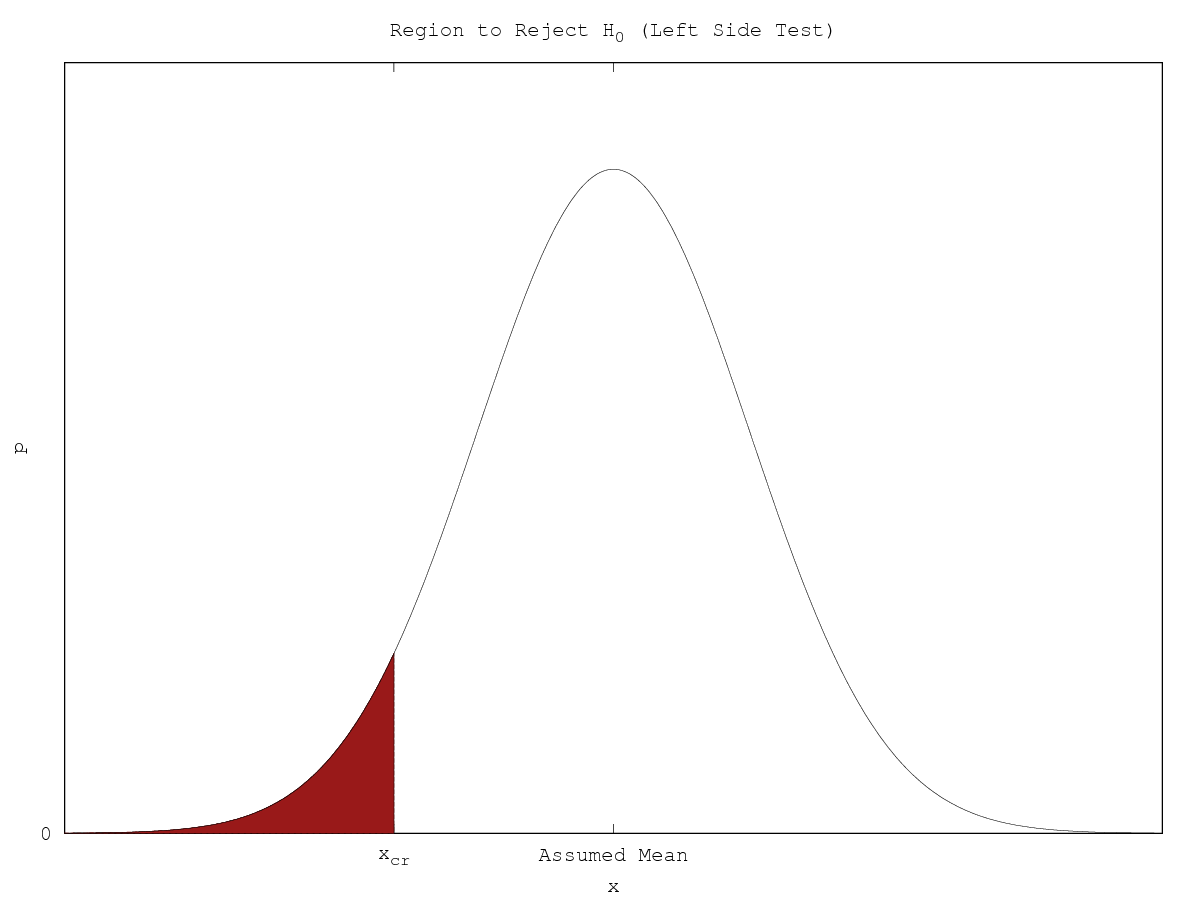
\includegraphics[width=5cm]{img/leftSideHypothesisTest}

  \end{columns}

  \begin{description}
  \item[$p$-value Approach:] The probability that you do worse than
    $\bar{x}$ is the area to the left under the curve. If the area is
    smaller than the significance level ($\alpha$) then it is an
    \textit{unlikely result}.
  \item[Classical Approach:] The area to the left of $x_{cr}$ is
    equal to the significance level ($\alpha$). If your $\bar{x}$ is
    less than this critical value then it is an \textit{unlikely
      result}.
  \end{description}


\end{frame}

\begin{frame}
  \frametitle{Right Sided Test of the Mean}

  \begin{columns}
    \column{0.45\textwidth}
    \textit{You think that the mean is higher.}

    Notation:
    \begin{eqnarray*}
      \begin{array}{lrcl}
        H_0: & \mu & = & \# \\
        H_a: & \mu & > & \#
      \end{array}
    \end{eqnarray*}

    \column{0.55\textwidth}

    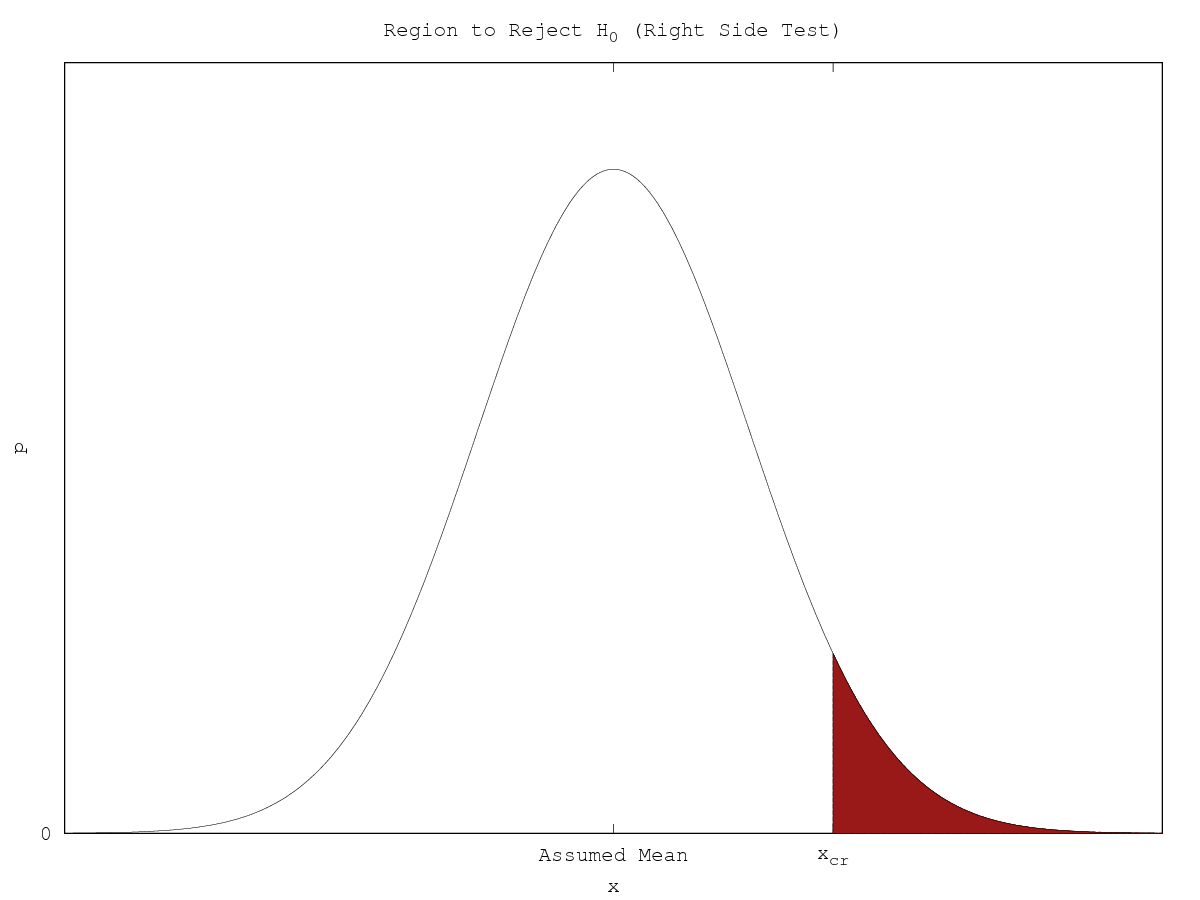
\includegraphics[width=5cm]{img/rightSideHypothesisTest}

  \end{columns}

  \begin{description}
  \item[$p$-value Approach:] The probability that you do worse than
    $\bar{x}$ is the area to the right under the curve. If the area is
    smaller than the significance level ($\alpha$) then it is an
    \textit{unlikely result}.
  \item[Classical Approach:] The area to the right of $x_{cr}$ is
    equal to the significance level ($\alpha$). If your $\bar{x}$ is
    more than this critical value then it is an \textit{unlikely
      result}.
  \end{description}


\end{frame}


\begin{frame}
  \frametitle{Two Sided Test of the Mean}

  \vspace*{-1em}

  \begin{columns}
    \column{0.45\textwidth}
    \textit{You think that the mean is different.}

    Notation:
    \begin{eqnarray*}
      \begin{array}{lrcl}
        H_0: & \mu & = & \# \\
        H_a: & \mu & \neq & \#
      \end{array}
    \end{eqnarray*}

    \column{0.55\textwidth}

    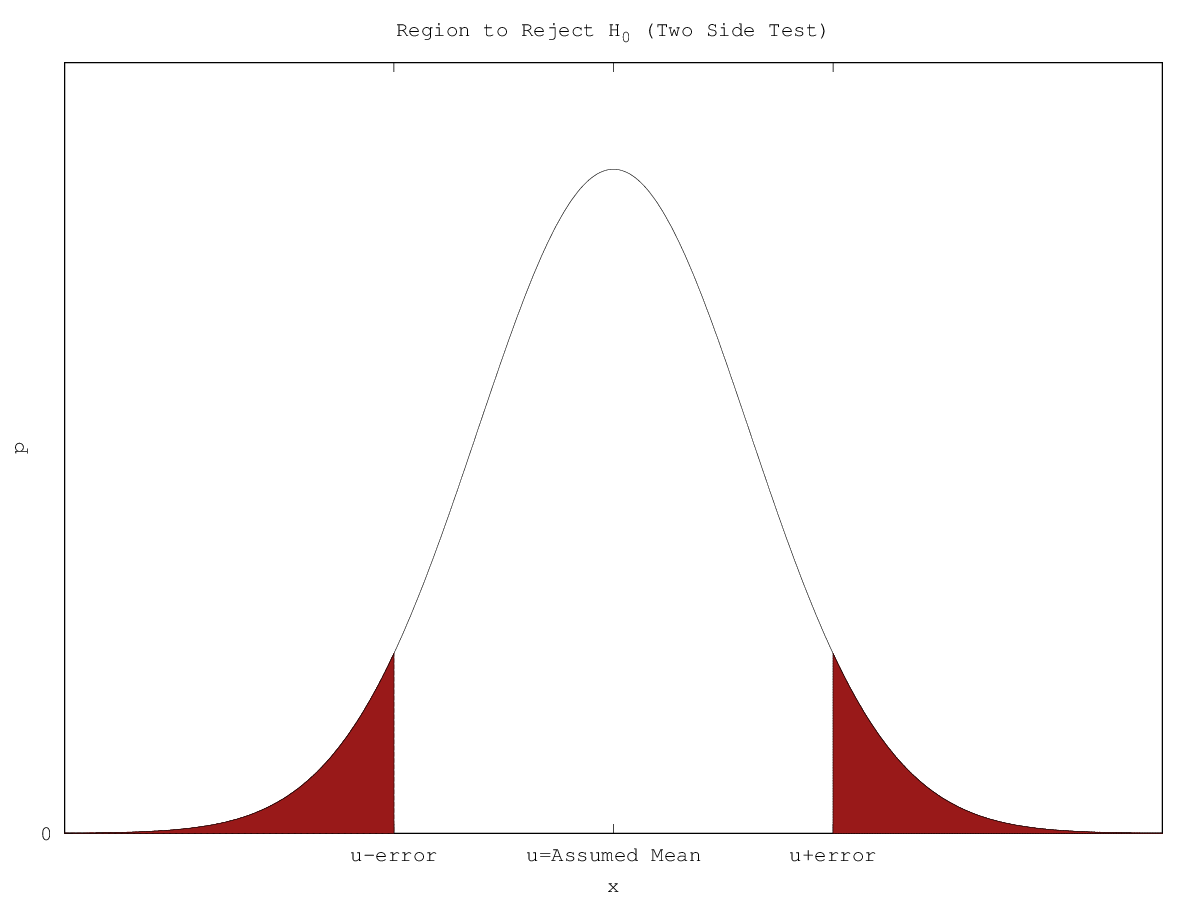
\includegraphics[width=5cm]{img/twoSideHypothesisTest}

  \end{columns}

  \begin{description}
  \item[$p$-value Approach:] The probability that you do worse than
    $\bar{x}$ is the area to the left \textit{and} right under the
    curve. If the area is smaller than the significance level
    ($\alpha$) then it is an \textit{unlikely result}.
  \item[Classical Approach:] The area to the left of
    $\mu-\mathrm{error}$ and to the right of $\mu+\mathrm{error}$ is
    equal to the significance level ($\alpha$). If your $\bar{x}$ is
    less than $\mu-\mathrm{error}$ or more than $\mu+\mathrm{error}$
    this critical value then it is an \textit{unlikely result}.
  \end{description}


\end{frame}



\begin{frame}{Example}

  A vendor claims that the spring constant for its springs is 0.040
  N/M. You suspect that the mean is really lower. You take a random
  sample of eight springs and find a sample mean of 0.038 N/m with a
  sample standard deviation of 0.0030 N/m. Use a confidence level of
  95\% to decide if your suspicions are correct.

  \vfill

  \only<2->
  {
    \begin{tabular}{l@{\hspace{2em}}l}
      $H_0$: & $\mu \geq 0.040$. \\
      $H_a$: & $\mu < 0.040$.
    \end{tabular}
  }

  \vfill

  \only<3-> { We cannot reject $H_0$ assuming a $t$-distribution with
    seven degrees of freedom and a 95\% confidence level.}

  \vfill

\end{frame}




\iftoggle{clicker}{%

  \begin{frame}{Clicker Quiz}

    A vendor claims that the company's lights have a mean voltage draw
    of 80V. You think that it is actually higher than that. What is
    the hypothesis test that you will use when you conduct a test?

    \begin{tabular}{l@{\hspace{2em}}l} \hline
      A \\
      $H_0$: & The mean voltage draw is less than 80V.\\
      $H_a$: & The mean voltage draw is more than 80V. \\
      \\  \hline
      B \\
      $H_0$: & The mean voltage draw is more than 80V. \\
      $H_a$: & The mean voltage draw is less than 80V. \\
      \\ \hline
      C \\
      $H_0$: & The mean voltage draw is not 80V.\\
      $H_a$: & The mean voltage draw is 80V. \\ \hline
    \end{tabular}

    
  \end{frame}

}


\begin{frame}{Problem}

  \vfill

  $\bar{x}$ is a random variable.

  \vfill

  The data can \textbf{lie}!

  \vfill
  
\end{frame}


\begin{frame}{The Possibilities}

  \centerline{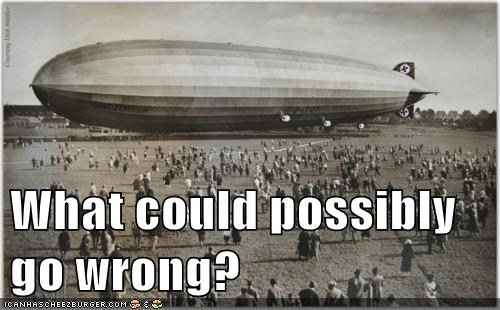
\includegraphics[width=6.0cm]{img/hindenburg}}

  \begin{eqnarray*}
    \mathrm{Data~-} & &
      \begin{array}{l@{\hspace{1em}}|c|c|} 
        \multicolumn{3}{r}{\mathrm{Reality}} \\ 
        \multicolumn{1}{c}{~} & \multicolumn{1}{c}{H_0
          \mathrm{~is~true}} & \multicolumn{1}{c}{H_0
          \mathrm{~is~false}} \\  
        \hhline{~--}
        \mathrm{Do~Not~Reject~}H_0 & 
\includegraphics[width=0.7cm]{img/smiley} & \mathrm{Type~II~Error} \\ \hhline{~|-|-|}
        \mathrm{Reject~}H_0 & \mathrm{Type~I~Error} & 
\includegraphics[width=0.7cm]{img/smiley} \\ \hhline{~--}
      \end{array}
  \end{eqnarray*}
  
\end{frame}


\begin{frame}{How To State Results}

  How you state your conclusions matter! It is an ethical issue in
  terms of conveying your assumptions and potential problems
  associated with the methodology.

  \begin{block}{Reject $H_0$}
    There is sufficient evidence to reject $H_0$ at the \#
    significance level assuming a $t$-distribution with \# degrees of
    freedom and a standard deviation of \#.
  \end{block}

  \begin{block}{Cannot Reject $H_0$}
    There is not sufficient evidence to reject $H_0$ at the \#
    significance level assuming a $t$-distribution with \# degrees of
    freedom and a standard deviation of \#.
  \end{block}

  
\end{frame}

\begin{frame}{The Methodology}

  What do we do?

  \begin{enumerate}
  \item Assume that $H_0$ is true.
  \item Ask, ``Are the data an unlikely result?''
  \end{enumerate}

  \uncover<2->
  {
    \begin{itemize}
    \item To reject $H_0$: The probability that we get our result must be ``small.''
    \item The probability that we get our result \textit{given our
        assumptions} is the significance level
      ($\alpha$). \textbf{\color{red} It is a conditional
        probability!}
    \end{itemize}
  }

  \uncover<3->
  {
    Note: We need to define this cut-off value, $\alpha$, \textbf{in
      advance!} i.e. before any data collection or manipulation.
  }
  
\end{frame}


% LocalWords:  Clarkson pausesection hideallsubsections
